%%% Group 4: Tahoe, Ksenia Sokolova, Xinmeng Tong
%%% Computational Physics
%%% Spring, 2017

%%%%%%%%%%%%%%%%%%%%%%%%%%%%%%%%%%%%%%%%%%%%%%%%%%%%%%%%%%%%%%%%%%%%%%%%%%%%%%%
%%% This code will develop a LaTeX'd writeup of the second group project
%%% assignment for PHYS566.
%%%%%%%%%%%%%%%%%%%%%%%%%%%%%%%%%%%%%%%%%%%%%%%%%%%%%%%%%%%%%%%%%%%%%%%%%%%%%%%%

% PACKAGES AND OTHER DOCUMENT CONFIGURATIONS
\documentclass[12pt]{article}
\usepackage[english]{babel}
\usepackage[utf8]{inputenc}
\usepackage{amsmath,amsfonts,amssymb}
\usepackage{graphicx,xcolor}
\usepackage{subfig}
\usepackage{booktabs,hyperref}
\usepackage[left=2cm,%
right=2cm,%
top=2cm,%
bottom=2cm,%
headheight=11pt,%
letterpaper]{geometry}%
\usepackage{fancyhdr}
\pagestyle{fancy}
\lhead{\small\sffamily\bfseries\leftmark}%
\chead{}%
\rhead{\small\sffamily\bfseries\rightmark}
\renewcommand{\headrulewidth}{1pt}
\renewcommand{\footrulewidth}{1pt}
\graphicspath{{images/}}

% Article Information
\title{Percolation of a 2D Lattice}
\author{Tahoe Schrader and Ksenia Sokolova \\PHYS566}
\date{}

% Begin writing document
\begin{document}
\maketitle

% Start with the abstract

\abstract{In this assignment we computationally explore various $2D$ lattices and generate their spanning clusters, $p_c$ and $\beta$. These variables refer to the probability a spanning cluster arises at and the critical exponent of a spanning cluster, respectively. Theoretically, these values for an infinite $2D$ lattice are $p_c\approx 0.593$ and $\beta=\frac{5}{36}=.138888$. Computationally, we were able to obtain $p_c = 0.594$ and a range $\beta=[.109436 \to 0.138344]$. These are reasonably close, which confirms that our code was successful.\\\\
Our code is available on GitHub: \\

\url{www.github.com/tahoeschrader/PHYS566_group4_projects}}

\section{Theory}
\label{sec:theory}
Percolation theory describes the behavior of connected clusters. This theory has many important relations to physics and chemistry. For example, it can be used to describe the movement and filtering of fluids through porous materials. When a system \emph{percolates}, a $2^\text{nd}$ order phase transition can also result.

The act of percolation refers to the existence of a spanning cluster. A spanning cluster is a cluster that reaches all edges of a physical boundary. For example, a spanning cluster must touch all four sides of a $2D$ box. Percolation, i.e. a system exhibiting a spanning cluster, is interesting because universality is \emph{also} exhibited. Universality is when the properties of the system are independent of the systems dynamical details.

One feature of the percolating system that we would like to document is the clustering probability, $p_c$, where generally
\begin{equation}
  \label{eq:probability}
  p = \frac{\text{\# of occupied lattice sites}}{\text{total lattice sites}}.
\end{equation}

Probability ranges and the theoretical results of such values are displayed in Table~\ref{table:pvalues}.
\begin{table}[!htb]
\centering{\minipage{0.75\textwidth}
  \centering{\begin{tabular}{ l | l }
    \hline
    small $p$ &  isolated clusters \\
    $p\approx 0.4$ &  many small clusters \\
    $p\approx 0.6$ &  large, barely connected clusters \\
    $p\approx 0.8$ &  most sites belong to same cluster \\
    \hline
  \end{tabular}}
  \caption{The physical representation of various occupation probabilities on a lattice.}
  \label{table:pvalues}
\endminipage}
\end{table}

Another important value in percolation theory is the fraction of all sites in the spanning cluster with respect to all occupied sites
\begin{equation}
  \label{eq:fraction}
  F = \frac{\text{\# of spanning sites}}{\text{total \# of cluster sites}}.
  \end{equation}
This value also takes the form
\begin{equation}
  \label{eq:spanningfraction}
  F = F_0 \left(p - p_c\right)^\beta,
\end{equation}
where $\beta$ is the critical exponent.

\subsection{2D Lattice Systems}
\label{sec:lattice}

The steps for generating a $2D$ percolating lattice are quite simple:
\begin{enumerate}
  \label{code:percolatinglattice}
  \item Generate a 2D lattice
  \item Populate a single lattice site at random and define it to be a cluster
  \item Populate another single lattice site at random
  \begin{enumerate}
    \item If the new site touches an old site, add it to the cluster
    \item If the new site doesn't touch an old site, define it to be a new cluster
    \item If the new site touches multiple different clusters, choose the smaller numbered cluster to ``win'' and overtake the other clusters
  \end{enumerate}
  \item Repeat until a spanning cluster arises
\end{enumerate}

It is evident that larger values of $p$ will more likely result in the existence of a spanning cluster than smaller values of $p$. Interestingly, the transmission from many clusters to a spanning cluster is sharp, qualifying it as a phase transition. For an infinite $2D$ lattice, the theoretical probability where this occurs is
\begin{equation}
  \label{eq:theoreticalpc}
  p_c \approx 0.593
\end{equation}
whereas the critical exponent of the spanning cluster fraction is
\begin{equation}
  \label{eq:theoreticalbeta}
  \beta = \frac{5}{36}.
\end{equation}

In Section~\ref{sec:results}, we computationally explore such a $2D$ lattice and generate spanning clusters, $p_c$ and $\beta$ for various lattice sizes.

\section{Results}
\label{sec:results}

\subsection{Extracting $p_c$}
\label{sec:pc}

First we determine the critical probability by running the code for $N=5, 10, 15, 20, 30, 50, 80$ for 50 times, every time finding the $p_c$.

To do this computationally, we used the cluster labeling method outlined above. Before running the averaging step, we tested the performance of our code by checking the dependencies between the time required to run one iteration and the size of the matrix. Please see results on Figure ~\ref{fig:timeElapsed}. Interestingly, these speeds are significantly faster than earlier version of our code. The time dependencies of an earlier version of our code can be seen in Figure~\ref{fig:timeElapsedOLD}. This speedup was achieved by removing nested for-loops in the spanning cluster check function, and by only generating new clusters where an old cluster did not already exist.

\begin{figure}[!htb]
\minipage{.5\textwidth}
  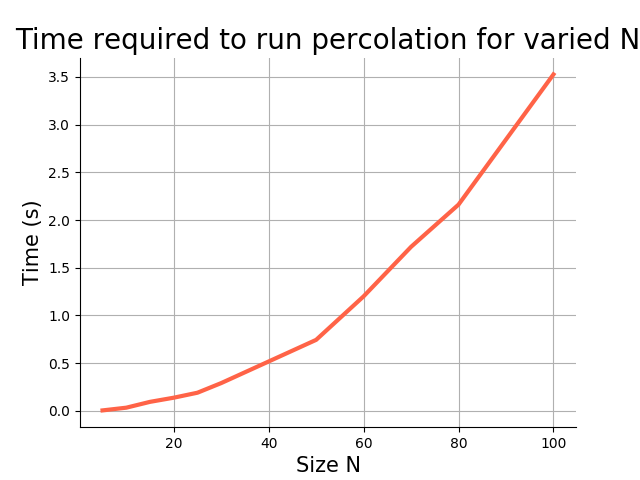
\includegraphics[width=\linewidth]{timeElapsedSPEEDY.png}
  \caption{Time elapsed and size of the matrix}\label{fig:timeElapsed}
\endminipage\hfill
\minipage{.45\textwidth}
  \includegraphics[width=\linewidth]{timeElapsed1.png}
  \caption{Time elapsed and size of the matrix for an earlier version of the code}\label{fig:timeElapsedOLD}
\endminipage\hfill
\end{figure}

We observe that our code is complexity $O[N^2]$, this is expected from the algorithm. This means that the larger the matrix, the worse the code performs, with squared scaling. And the change for the bad side happens relatively quickly. While this is durable for the cases we are observing, for larger matrices we would need to switch to a different algorithm.

Before the code calculates $p_c$, we can visually observe formation of clusters. (Note: on github project you can also find a .gif of the process). On the Figures ~\ref{fig:snapshotN30One} to ~\ref{fig:snapshotN30Spanning} we see the development of the cluster for $N=30$. In the beginning, as expected, we see many small clusters. As $p$ increases we observe formation of larger clusters, but still no spanning cluster. And at the end we see one large spanning cluster, and just a couple of smaller clusters.

\begin{figure}[!htb]
\minipage{0.3\textwidth}
  \includegraphics[width=\linewidth]{snapshotN30One.png}
  \caption{2D percolation start}\label{fig:snapshotN30One}
\endminipage\hfill
\minipage{0.3\textwidth}
  \includegraphics[width=\linewidth]{snapshotN30Two.png}
  \caption{2D percolation intermediate}\label{fig:snapshotN30Two}
\endminipage\hfill
\minipage{0.3\textwidth}
  \includegraphics[width=\linewidth]{snapshotN30Spanning.png}
  \caption{2D percolation spanning cluster}\label{fig:snapshotN30Spanning}
\endminipage\hfill
\end{figure}

To find critical probability, we ran the code for $N=5, 10, 15, 20, 30, 50, 80$ for 50 iterations, averaging for every N. The spanning clusters for these $N$ values are given in Figure~\ref{fig:N1} - \ref{fig:N7}.

\begin{figure}[!htb]
\minipage{0.3\textwidth}
  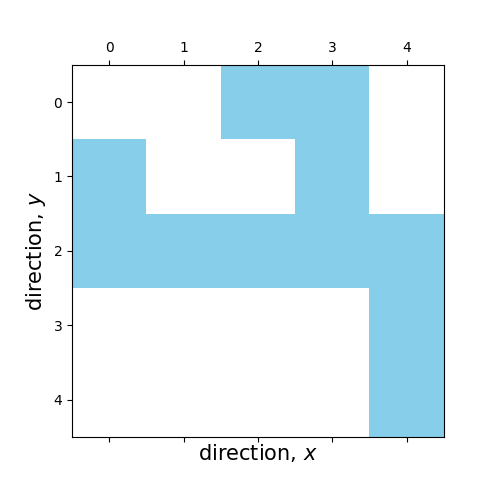
\includegraphics[width=\linewidth]{percolation5.png}
  \caption{2D percolation at $N=5$}\label{fig:N1}
\endminipage\hfill
\minipage{0.3\textwidth}
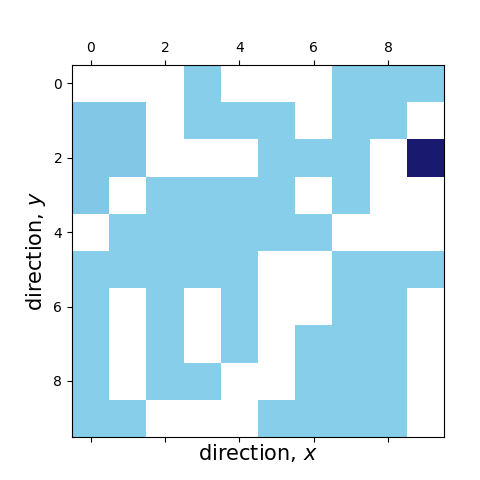
\includegraphics[width=\linewidth]{percolation10.png}
\caption{2D percolation at $N=10$}\label{fig:N2}
\endminipage\hfill
\minipage{0.3\textwidth}
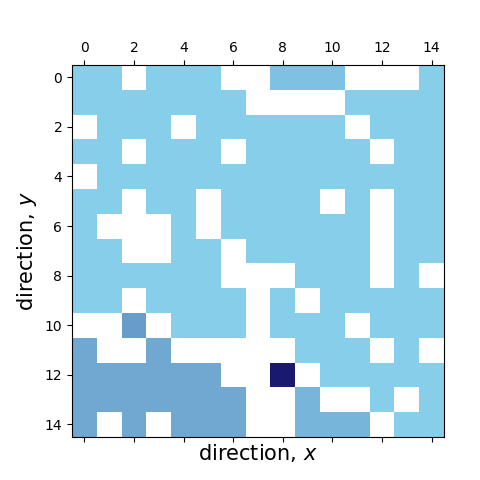
\includegraphics[width=\linewidth]{percolation15.png}
\caption{2D percolation at $N=15$}\label{fig:N3}
\endminipage\hfill \\
\minipage{0.3\textwidth}
  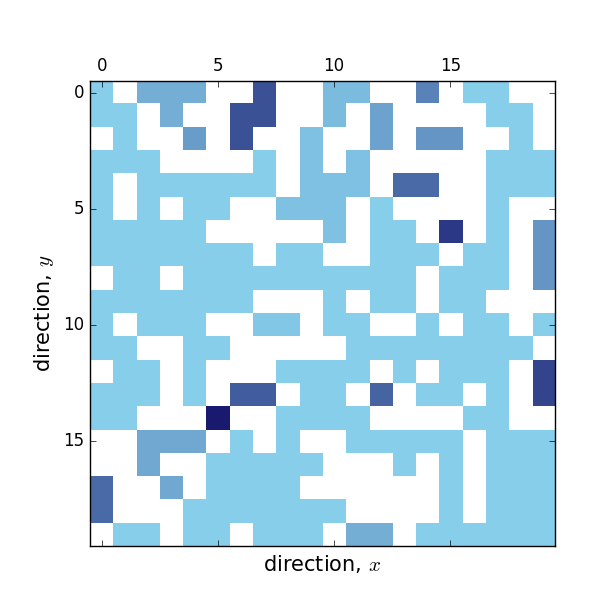
\includegraphics[width=\linewidth]{percolation20.png}
  \caption{2D percolation at $N=20$}\label{fig:N4}
\endminipage\hfill
\minipage{0.3\textwidth}
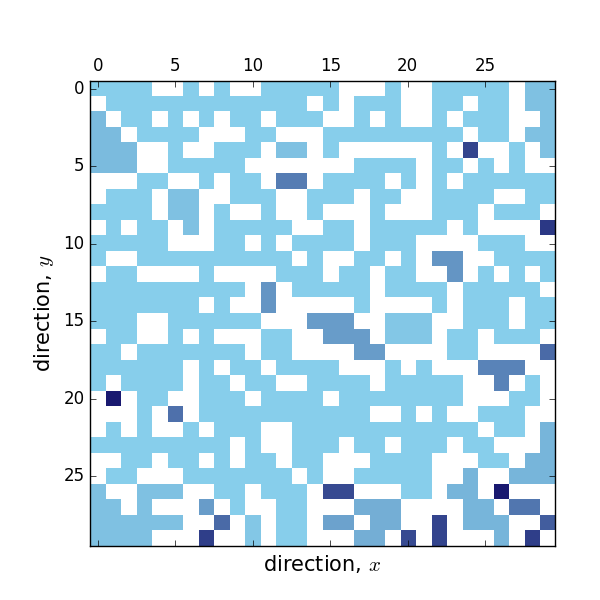
\includegraphics[width=\linewidth]{percolation30.png}
\caption{2D percolation at $N=30$}\label{fig:N5}
\endminipage\hfill
\minipage{0.3\textwidth}
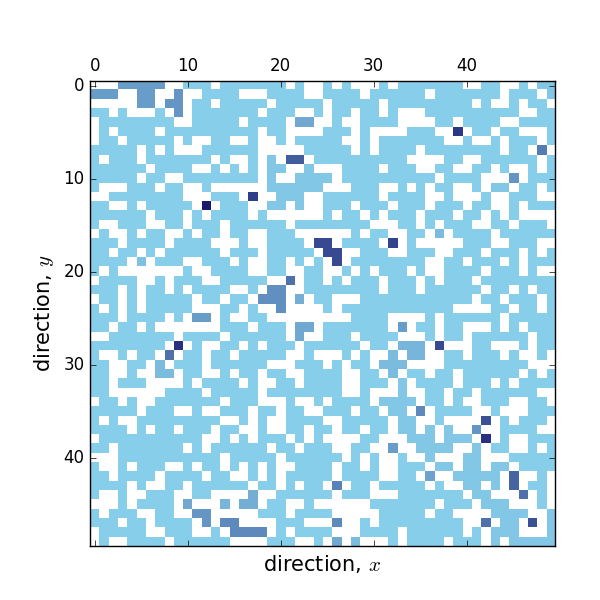
\includegraphics[width=\linewidth]{percolation50.png}
\caption{2D percolation at $N=50$}\label{fig:N6}
\endminipage\hfill \\
\centerline{\minipage{0.3\textwidth}
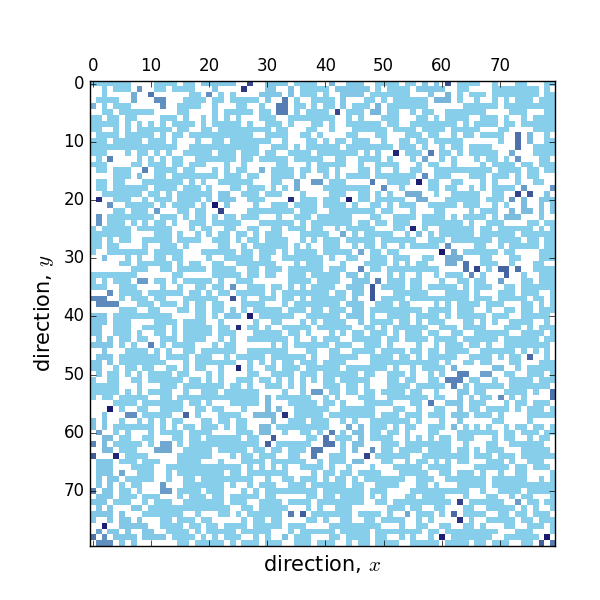
\includegraphics[width=\linewidth]{percolation80.png}
\caption{2D percolation at $N=80$}\label{fig:N7}
\endminipage}
\end{figure}

After extracting an average $p_c$ for each $N$, we extrapolated to find the critical probability. Please see the resulting plot attached (Figure ~\ref{fig:criticalProb}), which shows a critical probability of \textbf{$0.594$}. This is very close to the theoretical value of $0.593$.
\begin{figure}[!htb]
\centerline{\minipage{.7\textwidth}
  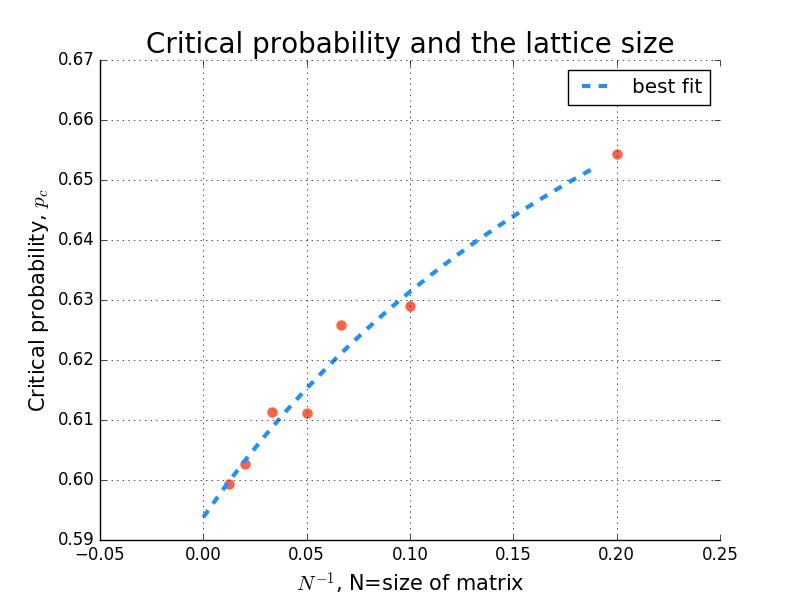
\includegraphics[width=\linewidth]{criticalProb0594.png}
  \caption{Critical probability plot for 2D percolation}\label{fig:criticalProb}
  \endminipage}
\end{figure}

\subsection{Extracting $\beta$}
\label{sec:beta}
Next, we fixed $N=100$ and computationally obtained parameter $\beta$.
To do so, we implemented the base code also used in part A. First, we reach the matrix with the spanning cluster (this was the result of running part a). Then, we add points one by one to the matrix, and record values F and p. F is calculated according the the formula:
\begin{equation}
    F=\frac{number \ sites\ in\ cluster}{total\ number\ occupied\ sites}
\end{equation}
And p is just the percent of occupied sites, or the concentration, if we consider the meaning of this parameter.

To speed up the calculations, we actually used some trick, like counting the total number of elements added as a counter, and not parsing though the matrix every step.

To average over all p, we had to make sure the vectors from each run are all the same length. The discrepancy in the length of the vectors for F and p from every of the 50 runs can arise from the randomness in the cluster formation. The concentration at which the spanning cluster was reached varies through every run. To avoid this error, we truncate the averages based on the highest $p_c$ achieved. We also average over all $p_c$ to make sure we can use the most precise value for finding $\beta$.

After we have found the averaged $p$ and $F$ values, we are looking for a power law of the form:
\begin{equation}
    F=F_0(p-p_c)^\beta
\end{equation}

This is true when $p$ is close to $p_c$, so we also take only first n values. We varied n to find the best amount of data to include. Experimentally, we found that leaving first 10\% of the $p$ and $F$ values provides a good agreement between theoretical and experimental $\beta$.

To find a fit for the $\beta$ we used a log transform:
\begin{equation}
    log(F)=log(F_0)+\beta*log(p-p_c)
\end{equation}

Please refer to the Figure \ref{fig:fraction100} and \ref{fig:fraction100log} for the plots.

We ran the code for the $N=100$ three times. The resulting $\beta$ were
\item 0.138344512943
\item 0.10943672863
\item 0.129361443917

Theoretical value of $\beta$ in decimal format is $0.1388889$

Therefore, our code consistently returned experimental $\beta$ close to the theoretical values. The visual inspection of the plots also showed good fits.

\begin{figure}[!htb]
\minipage{0.45\textwidth}
  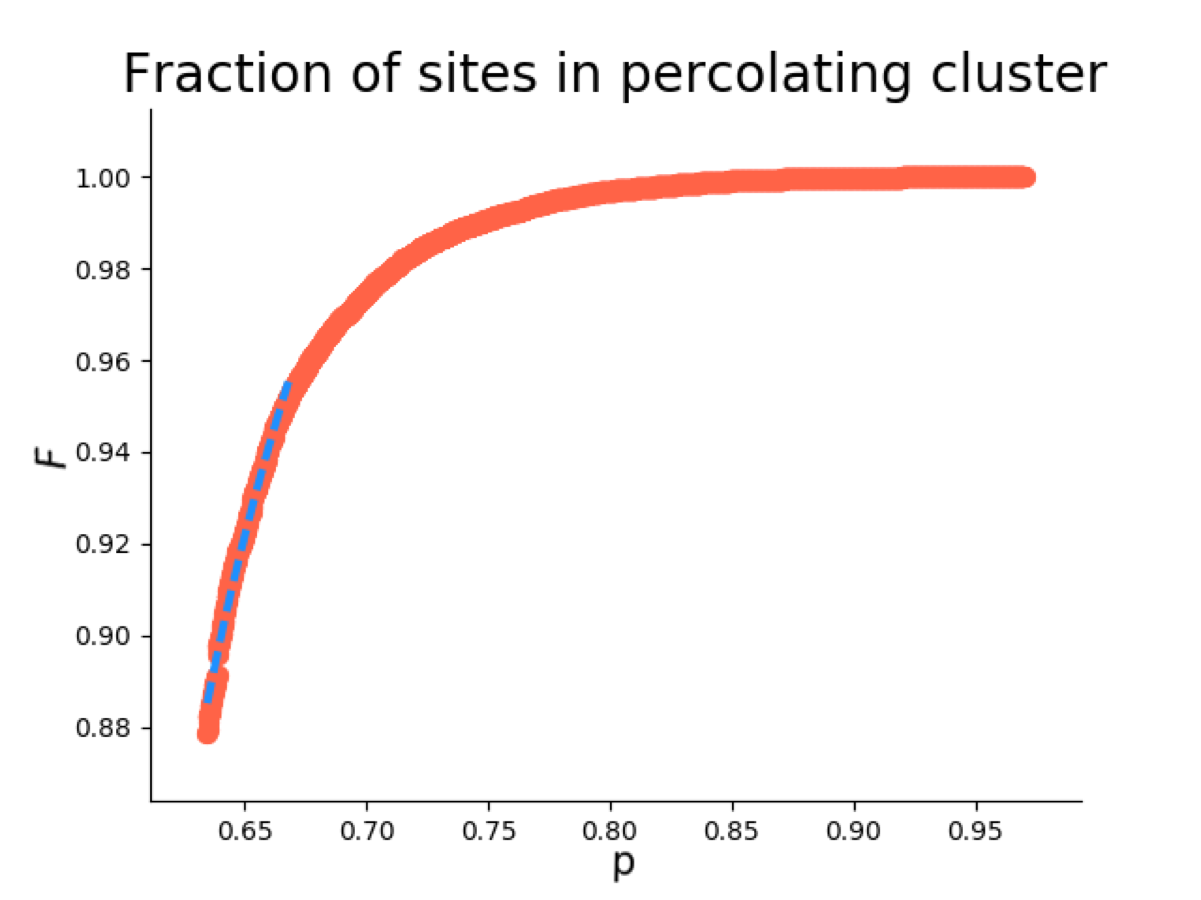
\includegraphics[width=\linewidth]{fractionFwithFit10percN100Axis.png}
  \caption{Fraction of sites in percolating cluster as function of concentration, N=100, average over 50 runs}\label{fig:fraction100}
\endminipage\hfill
\minipage{0.45\textwidth}
  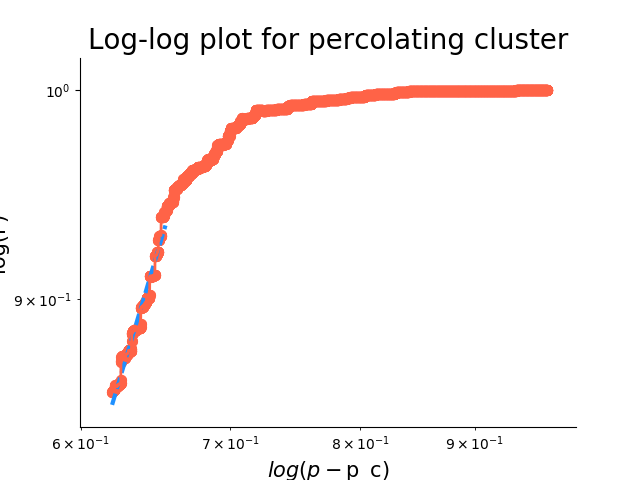
\includegraphics[width=\linewidth]{fractionFwithFit10percN100loglog.png}
  \caption{Fraction of sites in percolating cluster as function of concentration, N=100, average over 50 runs with log-log axes}\label{fig:fraction100log}
\endminipage\hfill
\end{figure}

\end{document}
